\subsection{Iteraciones de power method con y sin mejoras} 

\begin{figure}[!h]
        \begin{center}
                  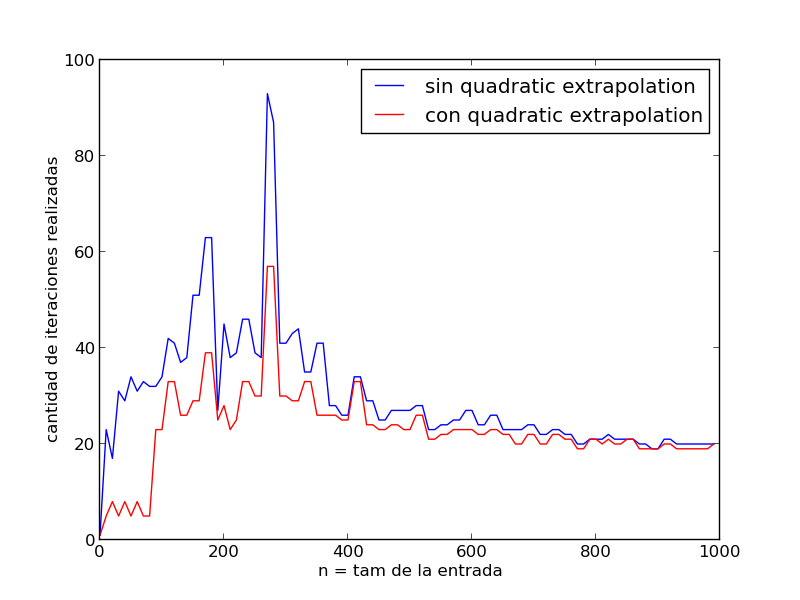
\includegraphics[scale = 0.6]{graficos/vs.png}
                  \caption{Iteraciones en función de cantidad de nodos}
                  \label{fig:contra1}
        \end{center}
\end{figure}
\FloatBarrier

El experimento fue realizado corriendo ambos algoritmos para 100 instancias de $i*10$ nodos,
con $0 \leq i \leq 99$.
Como podemos observar en la figura, la implementación que aplica Quadratic extrapolation realiza menos iteraciones
que la que no posee la optimización. Una particularidad que puede observarse consiste en que para valores mayores de $n$, la diferencia
la cantidad de iteraciones realizadas por ambos métodos disminuye.
